%caseBldg

In order to evaluate the control performance of our approach (SR-SQP) and compare it to R-SQP and SA, % of our method on a system with more meaningful dynamics than the point-mass system, 
we first test it on Heating, Ventilation and Air Conditioning (HVAC) control of a 4-state model of a single zone in a building. Such a model is commonly used in literature for evaluation of predictive control algorithms \cite{Jain2016}. The control problem we solve is similar to the example used in \cite{Raman14_MPCSTL}, where the objective is to bring the zone temperature to a comfortable range when the zone is occupied (given predictions on the building occupancy). The specification is:
\begin{equation}
\label{eq:BldgSpec}
\formula = \always_I(\text{ZoneTemp} \in \text{Comfort})
\end{equation}
Here, $I$ is the interval where the zone is occupied, and $\text{Comfort}$ is the range of temperatures (in Celsius) deemed comfortable ($[22,28]$). For the control horizon, we consider a 24 hour period, in which the building is occupied from time steps $10$ to $19$ (i.e. $I=[10,19]$), i.e. a 10-hour workday. 

\textbf{System dynamics.} The single-zone model, discretized at a sampling rate of 1 hour (which is common in building temperature control) is of the form:
\begin{equation}
\label{eq:bldg_dyn}
x_{k+1} = Ax_{k}+Bu_k+B_dd_k
\end{equation}
Here, $A$, $B$ and $B_d$ matrices are from the HAMLAB ISE model \cite{VanSchijndel2005}. $x \in \mathbb{R}^4$ is the state of the model, the $4^{th}$ element of which is the zone temperature, the others are auxiliary temperatures corresponding to other physical properties of the zone (walls and facade). The input to the system, $u \in \mathbb{R}^1$ is the heating/cooling energy to the system. $b_d \in \mathbb{R}^3$ are disturbances (due to occupancy, outside temperature, solar radiation), which we assume perfect predictions of. Data for the disturbances is obtained for $1^{st}$ April 2000, which is our 24 hours of interest, from \cite{VanSchijndel2005}. The control problem we solve is of the form in \eqref{eq:general_ctrl}, with $\gamma$ and $\delta$ both set to zero, and $X=[0,50]^4$, $U=[-1000,2000]$.
%i.e. robustness (smooth, when applicable) is only in the objective, to be maximized. This allows for a fair comparison between the three methods. 
%With respect to the general control problem of \eqref{eq:general_ctrl}, the limits on the states are $X=[0,50]^4$ and on the inputs $U=[-1000,2000]$.

\textbf{Results.} To initialize the optimization for all three methods, we generate an initial trajectory for the system \eqref{eq:bldg_dyn}, starting from $x_0=[21,21,21,21]'$, which does not satisfy $\formula$. The final trajectories after optimization from the three methods are shown in Fig.\ref{fig:ZoneTemp}. Our method (SR-SQP) and SA both result in trajectories that satisfy $\formula$, with a robustness of $2.9994$ and $2.8862$ respectively. On the other hand, R-SQP results in a trajectory that does not satisfy $\formula$ ($\rob_{\formula} = -0.1492$), and terminates on a local maxima. This is possibly due to the lack of existence of a gradient along certain directions, as seen in example \ref{ex:cluster nondiff}.

\textbf{Analysis.} In the particular problem, with the given comfort range, the maximum robustness achievable in the unconstrained case would $3$, achieved by setting the room temperature at $25$C for the interval $I$. SR-SQP results in a robustness which is just $0.02\%$ less than the unconstrained optimal value, while SA gets to a value $3.8\%$ less than the (unconstrained) optima. Note, for this particular problem, since we assume perfect knowledge of occupancy and disturbances, the problem of satisfying the formula, or indeed of even maximizing robustness, can be solved simply with a quadratic program with linear constraints. We use this example to illustrate the applicability of our method, as well as its performance, while adding a word of caution against the naive use of gradient descent for robustness maximization, even while the gradient of robustness exists \textit{almost everywhere}. In the following example, we take a specification which cannot be trivially turned into a quadratic-program. %without adding tighter constraints than the specification asks for (or binary variables).


\begin{figure}[t]
\centering
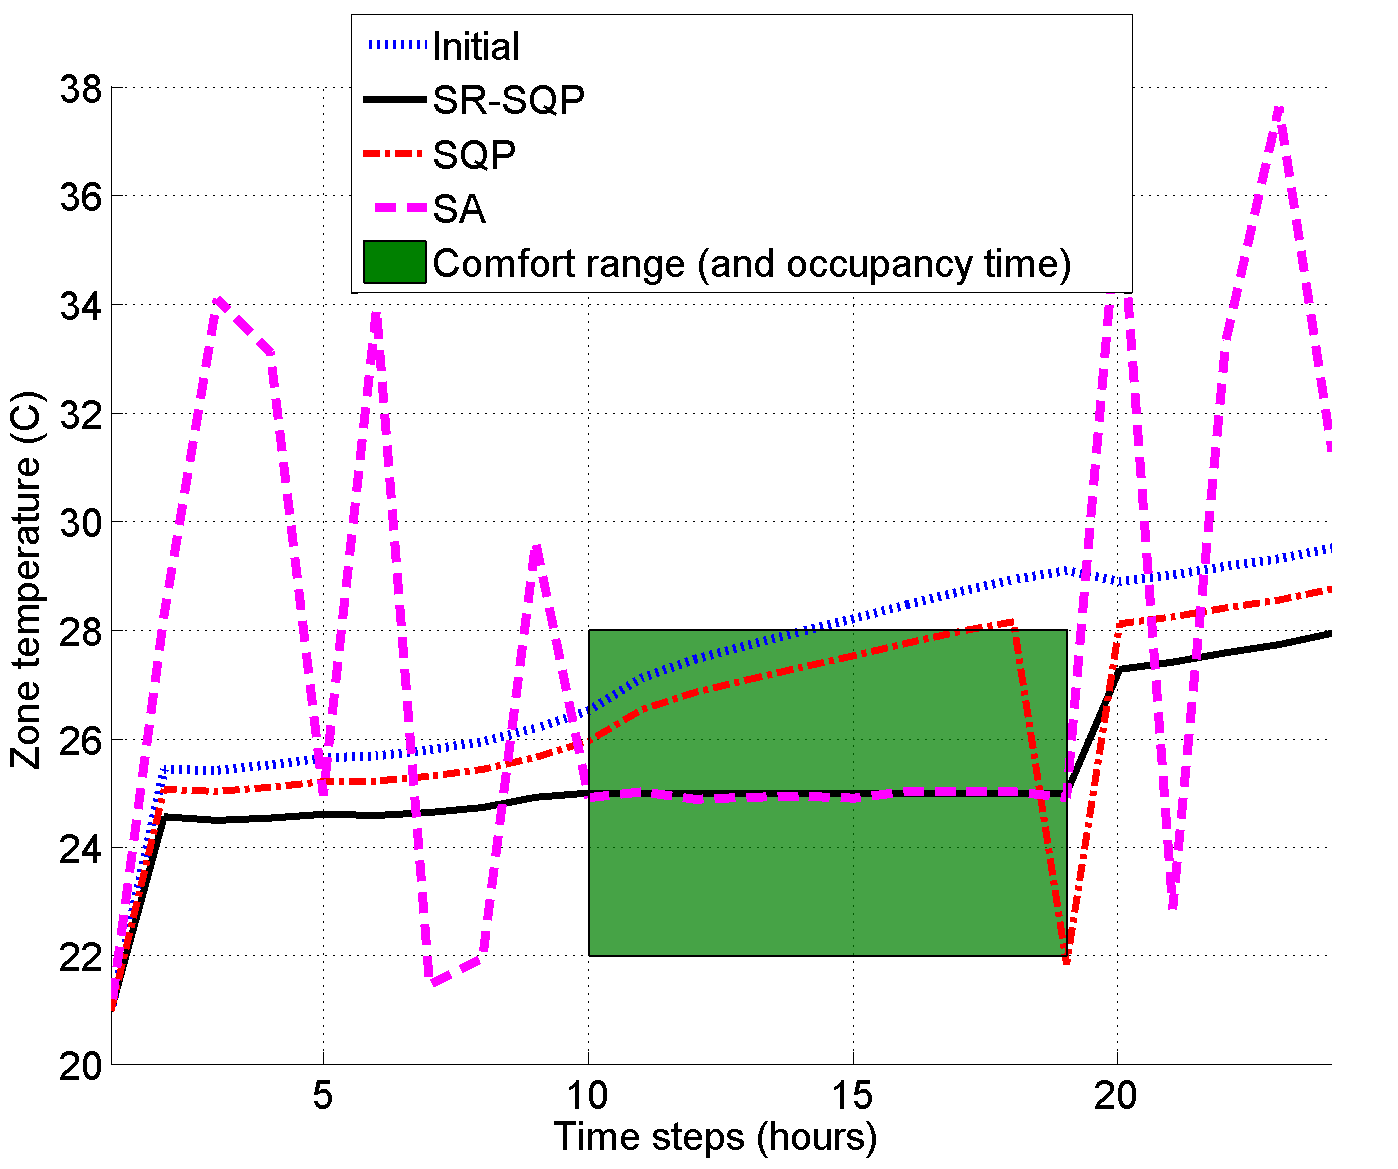
\includegraphics[width=0.49\textwidth]{figures/ZoneTemp_scissored}
\vspace{-20pt}
\caption{\small{Zone temperatures. The green rectangle shows the comfortable temperature limit of 22-28 C, applicable during time steps 10-19 (when the building is occupied).}}
\label{fig:ZoneTemp}
\vspace{-10pt}
\end{figure}

%1. Single zone building model from ...

%2. Specification for comfort when occupied.

%3. 24 hour look ahead, given disturbances and occupancy. Initial guess (with negative robustness) via solving an LP.

%4. Can be applied in a receding horizon manner. For the given setting, could very well be solved using a linear program asking for temperature between 22-28C for time steps 10 to 19, but we use our method to illustrate how robustness based control can be used to satisfy a specification. The next example (Autonomous ATC) shows control with a specification cannot be trivially translated to a linear program with Polyhedral constraints.

%5. Figure shows room temperature for the 3 methods (other states and disturbances/control in a single figure if necessary)

%6. Table shows robustness of obtained trajectory via the 3 methods. Note, Optimal solution would be temperature of 25C  (robustness of 3) for the occupancy period (if dynamics/constraints would allow it).
